\documentclass[a4paper,12pt]{report}
\usepackage{graphics}
\usepackage{amsmath}
\usepackage{amssymb}
\usepackage{array}
\usepackage{longtable}
\usepackage{textcomp}
%\usepackage[dark,first,bottomafter]{draftcopy}


\setlength{\LTcapwidth}{6in}

\title{The Juicer LVCSR Decoder - User Manual{\newline}\vspace{5mm}{\Large for Juicer version ***VER***}} 
\author{Darren Moore \\
IDIAP Research Institute \\
Martigny, Switzerland. \\
{\tt moore@idiap.ch}
}
\date{October 26, 2005}

\begin{document}
\maketitle
\tableofcontents


%%%%%%%%%%%%%%%%%%%%%%%%%%%%%%%%%%%%%%%%%%%%%%
\chapter{Introduction}

\section{Overview}

Juicer is a decoder for HMM-based large vocabulary speech recognition that uses
a weighted finite state transducer (WFST) representation of the search space. The package
consists of a number of command line utilities: the Juicer decoder itself, along
with a number of tools and scripts that are used to combine the various ASR
knowledge sources (language model, pronunciation dictionary, acoustic models)
into a single, optimised WFST that is input to the decoder. The Juicer package is distributed under a BSD license (see Appendix~\ref{app:license}).

The major advantages of the WFST-based approach is the decoupling of the decoding network from the decoding engine, as well as a common representation of the various ASR knowledge sources allowing standardised techniques to be used for constructing a complete, optimised search space. These characteristics allow straightforward incorporation of new capabilities, such as decoding with a custom grammar or non-standard lexical constraints, without requiring modification of the decoding engine.

An overview of Juicer is illustrated in Figure~\ref{fig:juicerarch}.

\begin{figure}
\begin{center}
\resizebox{16cm}{!}{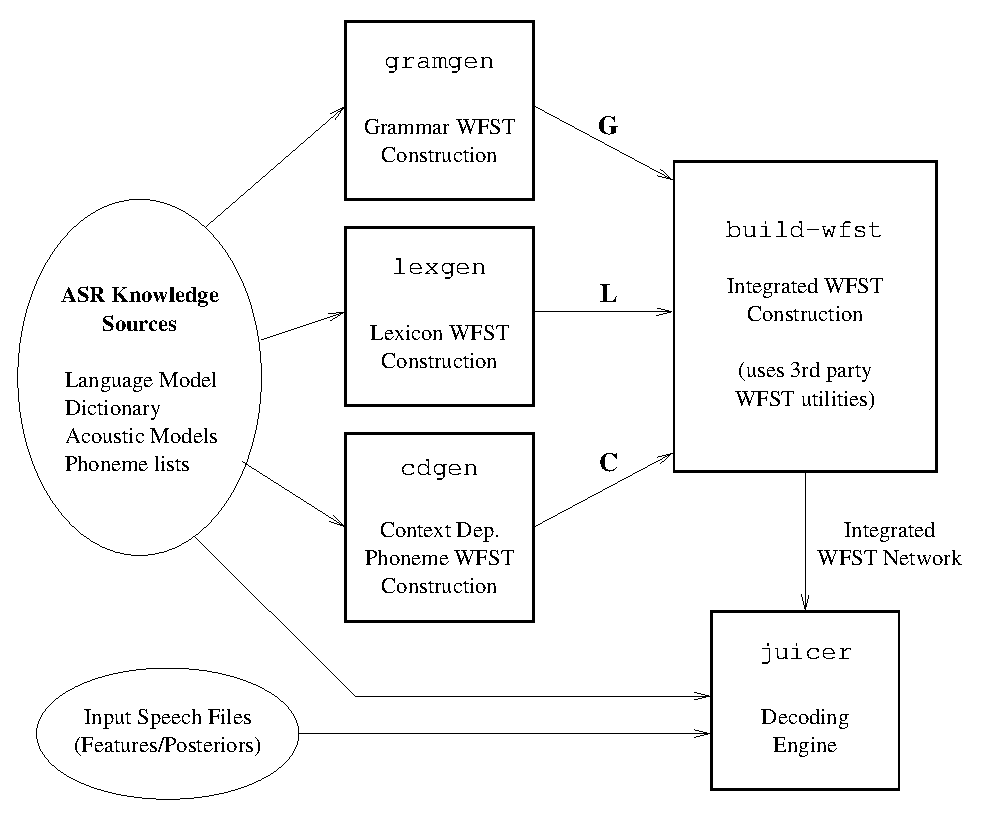
\includegraphics{pics/juicer_arch.eps}}
\caption{High level architecture of the Juicer decoding package}
\label{fig:juicerarch}
\end{center}
\end{figure}

This document contains detailed instructions for use. Those wishing to attempt a ``quick start'' can skip to Chapter~\ref{chap:examples} and examine the example systems and decoding configurations provided.

\section{Current capabilities}

\begin{itemize}
\item Language Modelling
\begin{itemize}
   \item simple word-loop with start/end silence
   \item word-pair grammar
   \item $N$-gram (arbitrary $N$, subject to memory limitations - see Chapter~\ref{chap:limitations})
\end{itemize}
\item Acoustic Modelling
\begin{itemize}
   \item monophones
   \item word-internal $n$-phones (tri/quin/...)
   \item cross-word triphones
   \item HTK MMF file format support
\end{itemize}
\item Dictionary
\begin{itemize}
   \item multiple pronunciations of same word
   \item pronunciation probabilities
\end{itemize}
\item Decoding Search
\begin{itemize}
   \item Flexible WFST-based decoder (decoding network independent of decoding engine implementation)
   \item Viterbi search
   \item Beam-search pruning (global, model-end)
   \item Histogram pruning
   \item Lattice generation
   \item Word-level or model-level output
\end{itemize}
\item Other
\begin{itemize}
   \item Hybrid HMM/ANN decoding supported (using LNA-format posterior files).
\end{itemize}
\end{itemize}


%%%%%%%%%%%%%%%%%%%%%%%%%%%%%%%%%%%%%%%%%%%%%%
\chapter{Installation}
\label{chap:installation}

% prerequisites


\begin{itemize}
\item Copy.
\begin{enumerate}
   \item Create a directory, {\tt <dir>}, for juicer (e.g. {\tt /home/moore/juicer})
   \item {\tt cp /home/speech/moore/juicer\_rel/juicer-***VER***.tar.gz <dir>}
\end{enumerate}
\item Extract files.
\begin{enumerate}
   \item {\tt cd <dir>}
   \item {\tt tar -xzvf juicer-***VER***.tar.gz}
\end{enumerate}
\item Build Juicer tools.
\begin{enumerate}
   \item {\tt cd <dir>/code/tools}
   \item {\tt make}
   \item Try running tools as a test for build success (e.g. {\tt ./cdgen -h})
\end{enumerate}
\item Build MIT FST toolkit.
\begin{enumerate}
   \item {\tt cd <dir>/tools/mitfst-1.0.0/src/lib}
   \item {\tt make}
   \item {\tt cd ../tools}
   \item {\tt make}
   \item Try running tools as a test for build success (e.g. {\tt ../../bin/fst\_info})
\end{enumerate}
\item Obtain AT\&T FSM toolkit version $4.0$.
\begin{enumerate}
   \item Download from {\tt http://www.research.att.com/sw/tools/fsm/}
   \item Install in a directory, {\tt <fsmdir>}, of your choice.
\end{enumerate}
\item Configure juicer environment file.
\begin{enumerate}
   \item edit {\tt <dir>/code/tools/juicer-env.csh}
   \item modify {\tt JUTOOLS} path to be absolute path of {\tt <dir>/code/tools}
   \item modify {\tt ATTFSMDIR} path to be absolute path of {\tt <fsmdir>/bin}
\end{enumerate}
\end{itemize}


%%%%%%%%%%%%%%%%%%%%%%%%%%%%%%%%%%%%%%%%%%%%%%
\chapter{Instructions for use}

Decoding with Juicer involves 3 main steps :

\begin{enumerate}
\item Generate 3 individual WFST's (LM, lexicon, phoneme).
\item Build integrated WFST from individual WFST's.
\item Run Juicer decoder.
\end{enumerate}

\section{WFST generation}

This section describes the three tools: {\tt gramgen}, {\tt lexgen}, and {\tt cdgen} that are used to transform the ASR knowledge sources into weighted finite-state transducer representations. The output of each of these tools is 3 files: an FSM format file~\cite{attfsmformats} containing the WFST itself, along with input and output symbols files that map from the numerical labels in the FSM file to the relevant string representations (words, phoneme names, etc).

It is important to maintain consistency in the files and options that are passed to these tools, and subsequently to the juicer decoder. For example, the {\tt lexgen} and {\tt cdgen} tools as well as the {\tt juicer} decoder all have a {\tt -monoListFName} option. The same monophone list file must be passed to all these tools for correct operation.

One rudimentary check that consistency has been preserved between the {\tt gramgen} and {\tt lexgen} tools is to compare the output symbols file generated with {\tt gramgen} to the input symbols file generated with {\tt lexgen}. These two symbols files should be identical. The same comparison can be done with the output symbols file from {\tt lexgen} and the input symbols file from {\tt cdgen}.


\subsection{Grammar WFST}

The grammar WFST is generated using the {\tt gramgen} executable, which can be found in the tools directory after the source code has been successfully built. The purpose of the grammar WFST is to ensure that sequences of recognised words conform to the grammar or language model.

The command-line help (obtained by executing {\tt gramgen -h}) is displayed in Figure \ref{fig:gramgen_help}. Basically, the user inputs a dictionary (defining the set of words to recognise), the type of grammar to use, and depending on the grammar type, a file containing the grammar definition (e.g. an ARPA LM file when the grammar type is {\tt ngram}). The tool then outputs a WFST in AT\&T FSM format, together with input and output symbol files.

The tool is capable of producing grammar WFST's of the following types:
\begin{itemize}
\item Simple word loop, with sentence marker words at beginning and end.
\item Word-pair grammar.
\item N-gram language model.
\end{itemize}

The desired word insertion penalty and language model scaling factor are specified during grammar WFST construction. These parameters cannot be specified when invoking the decoder.

The {\tt gramgen} command line options are described in detail in Table~\ref{tab:gramgen_ref}.

\begin{figure}
\begin{center}
\resizebox{16cm}{!}{\includegraphics{pics/gramgen.epsi}}
\caption{Command line help message for the {\tt gramgen} tool.}
\label{fig:gramgen_help}
\end{center}
\end{figure}

\begin{center}
\begin{longtable}{lp{9cm}}
%%%% First header
\caption{Detailed description of {\tt gramgen} command line options.} \\
\label{tab:gramgen_ref} \\
\hline
Option & Description \\
\hline
\endfirsthead
%%%% All headers except first
\caption{(continued)} \\
\hline
Option & Description \\
\hline
\endhead
%%%% All footers
\hline
\endfoot
%%%% Table body
{\tt -lexFName \emph{string}} & {\bf Required.} The name of the text file containing the pronunciation dictionary. \\
{\tt -sentStartWord \emph {string}} & The word in the dictionary that begins every recognised sentence (e.g. {\tt <s>}). Note: this option is mandatory for grammar types {\tt silwordloopsil} and {\tt wordpair}. \\
{\tt -sentEndWord \emph{string}} & The word in the dictionary that ends every recognised sentence (e.g. {\tt </s>}). Note: this option is mandatory for grammar types {\tt silwordloopsil} and {\tt wordpair}. \\
{\tt -lmFName \emph{string}} & The file containing the original grammar specification for grammar types of {\tt ngram} and {\tt wordpair}. N-gram LM files are expected to be in standard ARPA-MIT format (see Section 16.7.1 of~\cite{htkbook321}). Word pair grammar files are expected to be in the BBN word pair grammar format as used in the ARPA Navel Resource Management task. Note: the option is mandatory for grammar types {\tt ngram} and {\tt wordpair}, and is ignored otherwise. \\
{\tt -lmScaleFactor \emph{float}} & All LM probabilities from the original grammar specification are converted to natural log, and are then multiplied by this value. The scaled values are used in the output WFST. The purpose of this parameter is to bring LM weights into line with acoustic model output likelihoods (which are typically grossly under-estimated), and also to control the importance of the acoustic models relative to the language model. This option is ignored for grammar type {\tt silwordloopsil}. Default value if omitted is $1.0$. \\
{\tt -wordInsPen \emph{float}} & This is a natural log value that is added to each LM probability (after scaling). The general effect of varying this parameter is to tradeoff between the insertion and deletion rates in the final decoder output. Note that the LM scaling factor also affects insertion and deletion rates. Default value if omitted is $0.0$. \\
{\tt -unkWord \emph{string}} & This only applies when grammar type is {\tt ngram} and specifies the unknown word in the ARPA LM file (e.g. {\tt <unk>}). All dictionary words that are not present in the LM are mapped to the unknown word for the purpose of determining LM probabilities. Note that an error occurs if there are words in the LM that are not in the dictionary. \\
{\tt -gramType \emph{string}} & {\bf Required.} This specifies the type of the grammar that is to be output. Permissible grammar types are {\tt silwordloopsil}, {\tt ngram}, and {\tt wordpair}. \\
{\tt -fsmFName \emph{string}} & {\bf Required.} The filename of the output grammar WFST file. This file is in AT\&T FSM format~\cite{attfsmformats}. \\
{\tt -inSymsFName \emph{string}} & {\bf Required.} The filename of the input-symbols file that corresponds to the output WFST file. The entries in this file map from the numeric labels used in the FSM file to actual word strings. \\
{\tt -outSymsFName \emph{string}} & {\bf Required.} The filename of the output-symbols file that corresponds to the output WFST file. The entries in this file map from the numeric labels used in the FSM file to actual word strings. Note that for all grammar types currently implemented, the output-symbols file will be identical to the input-symbols file. \\
{\tt -genTestSeqs} & When specified, some debug sequences are output using the WFST after it is constructed, which is useful to confirm its correctness.
\label{tab:gramgen_options}
\end{longtable}
\end{center}

\subsection{Lexicon transducer}
\label{sec:lexgen}

The lexicon transducer is generated using the {\tt lexgen} tool, which can be
found in the tools directory after the source code has been successfully built.
The lexicon transducer maps sequences of monophones (or more precisely, the
sub-word units used in the pronunciation dictionary) to sequences of words. Any
weights present in the final WFST are due to probabilities assigned to
pronunciations.

The command-line help (obtained by executing {\tt lexgen -h}) is displayed in Figure~\ref{fig:lexgen_help}. 
The {\tt lexgen} command line options are described in detail in Table~\ref{tab:lexgen_ref}.


\begin{figure}
\begin{center}
\resizebox{16cm}{!}{\includegraphics{pics/lexgen.epsi}}
\caption{Command line help message for the {\tt lexgen} tool.}
\label{fig:lexgen_help}
\end{center}
\end{figure}

\begin{center}
\begin{longtable}{lp{9cm}}
%%%% First header
\caption{Detailed description of {\tt lexgen} command line options.} \\
\label{tab:lexgen_ref} \\
\hline
Option & Description \\
\hline
\endfirsthead
%%%% All headers except first
\caption{(continued)} \\
\hline
Option & Description \\
\hline
\endhead
%%%% All footers
\hline
\endfoot
%%%% Table body
{\tt -lexFName \emph{string}} & {\bf Required.} The name of the text file containing the pronunciation dictionary. Each line of this file is in the standard dictionary format ``{\tt word(prob) ph1 ph2 ... phN}'' where the pronunciation probability, ``{\tt (prob)}'', is optional. Do not specify multiple pronunciations of the same word with silence or short-pause phones at the end, as this is achieved with the {\tt -addPronunsWithEndSil} and {\tt -addPronunsWithEndPause} options described below. \\
{\tt -sentStartWord \emph {string}} & The word in the dictionary that begins every recognised sentence (e.g. {\tt <s>}). The sentence start word is immune from the effects of the {\tt -addPronunsWithEndSil} and {\tt -addPronunsWithEndPause} options (i.e. no additional pronunciations are added). \\
{\tt -sentEndWord \emph{string}} & The word in the dictionary that ends every recognised sentence (e.g. {\tt </s>}). The sentence end word is immune from the effects of the {\tt -addPronunsWithEndSil} and {\tt -addPronunsWithEndPause} options (i.e. no additional pronunciations are added). \\
{\tt -monoListFName \emph{string}} & {\bf Required.} The name of a text file containing the complete list of unique phonemes (one phoneme per line) that are used in the dictionary, and elsewhere in the system (e.g. to form context dependent phone names). \\
{\tt -silMonophone \emph{string}} & The name of the silence phoneme, which must be present in the monophone list file. Mandatory if {\tt -addPronunsWithEndSil} is specified, ignored otherwise. \\
{\tt -pauseMonophone \emph{string}} & The name of the pause phoneme, which must be present in the monophone list file. Mandatory if {\tt -addPronunsWithEndPause} is specified, ignored otherwise. \\
{\tt -pauseTeeTransProb \emph{float}} & The (non-log) initial-to-final state transition probability for the pause model. This is ignored unless {\tt -addPronunsWithEndPause} is specified. If a value $>0$ is defined then that value is used as the probability for the ``base'' pronunciation (i.e. without silence or pause at the end), and $1-$ the value is used as the probability of the pronunciation with pause at the end. See Section~\ref{sec:lexgen} for a more detailed discussion about this. \\
{\tt -fsmFName \emph{string}} & {\bf Required.} The filename of the output lexicon WFST file. This file is in AT\&T FSM format. \\
{\tt -inSymsFName \emph{string}} & {\bf Required.} The filename of the input-symbols file that corresponds to the output WFST file. The entries in this file map from the numeric labels used in the FSM file to the names in the monophone list file. \\
{\tt -outSymsFName \emph{string}} & {\bf Required.} The filename of the output-symbols file that corresponds to the output WFST file. The entries in this file map from the numeric labels used in the FSM file to the word strings in the dictionary. \\
{\tt -addPronunsWithEndSil} & Include an additional pronunciation for each word in the dictionary with the silence phoneme (specified with the {\tt -silMonophone} option) added to the end. The sentence start word and sentence end word are not affected. \\
{\tt -addPronunsWithEndPause} & Include an additional pronunciation for each word in the dictionart with the pause phoneme (specified with the {\tt -pauseMonophone} option) added at the end. The sentence start and sentence end word are not affected. Note that the {\tt -pauseTeeTransProb} option affects pronunciation probabilities when this flag is defined. \\
\end{longtable}
\end{center}


\subsubsection{Dictionary file format}

The dictionary/lexicon file is a text file with one entry per line. The format of each line is:

\vspace{5mm}
{\tt word(prior) ph1 ph2 $\dots$ phN}
\vspace{5mm}

where {\tt(prior)} is the optional pronunciation prior probability (non-log), and {\tt ph1 ph2 $\dots$ phN} are the sub-word units that define the pronunciation of {\tt word}. The sub-word units used in the dictionary are the same sub-word units in the monophone list file that is input to {\tt lexgen} and other tools. Any amount of whitespace can be used to separate the fields.

Multiple (different) pronunciations of the same word are permitted. If pronunciation probabilities are omitted, then a probability of $1.0$ is assumed, even in the multiple pronunciation case.

{\bf Do not} add multiple pronunciations in the dictionary for the same word with additional silence or pause phones at the end, as this is achieved using the {\tt -addPronunsWithEndSil} and {\tt -addPronunsWithEndPause} options described in Table~\ref{tab:lexgen_ref}.

There is no requirement for the dictionary to be correctly sorted.


\subsubsection{Silence handling}

Silence at the start and end of utterances is accommodated by adding sentence start and end words to the dictionary (e.g. {\tt <s>} and {\tt </s>}) that contain only the silence monophone in their pronunciation. The sentence start and sentence end words should match any sentence markers that occur in the language model. These words are then specified to both the WFST construction tools and to the decoder using the {\tt -sentStartWord} and {\tt -sentEndWord} options. When using this configuration, silence at the start and end of all utterances is assumed, and the decoder output for each utterance will always begin with the sentence start word and finish with the sentence end word.

Between-word silence is allowed by defining two pronunciations for each dictionary entry. The first pronunciation is the one defined in the lexicon file. The second pronunciation is the same as the first, except with the silence monophone (as specified with the {\tt -silMonophone} option) added to the end of the entry. The second pronunciation is not explicitly defined in the lexicon file, but is included automatically with the {\tt -addPronunsWithEndSil} option. The sentence start and end words are not affected by the {\tt -addPronunsWithEndSil} option. This method assumes that silence occurs only at the end of words. Appropriate part-words must be added to the dictionary if within-word silence is to be handled during decoding.

Silence is always treated as context independent. This means that there must be a HMM defined for the silence monophone. In a cross-word triphone system, the integrated transducer accepts input sequences such as: {\tt sil sil-k+ae k-ae+t ae-t+sil sil} \footnote{Note that in such cross-word systems where the only context independent phoneme models are silence and (perhaps) short-pause, this implies that all utterances must begin and end with silence, which further implies that the first monophone in the sentence start word pronunciation must be silence, and the final monophone in the sentence end word pronunciation must be silence.}. In the word-internal $n$-phone case, where the ``monophones'' are in fact the context dependent phonemes used in the dictionary, the integrated transducer accepts input sequences such as: {\tt sil k+ae k-ae+t ae-t sil}.


\subsubsection{Pause handling}

Often it is desirable to model the presence of short pauses between words separately to the modelling of more general silence conditions. Similar to the handling of silence above, the transducer construction tools allow a pause monophone to be specified (using the {\tt -pauseMonophone} option), and an additional pronunciation with pause at the end can be added automatically for each dictionary entry using the {\tt -addPronunsWithEndPause} option with {\tt lexgen}.

However, usually the HMM for pause (particularly when built using HTK) contains a transition from the initial non-emitting state to the final non-emitting state (HTK refers to such HMM's as \emph{tee} models). The addition of this pause model to the end of each pronunciation models the presence of an \emph{optional} short pause between words. 

{\bf Juicer cannot decode with HMM's that contain this initial-final state transition}. However, the optional pause functionality is retained firstly through the addition of the pronunciation with pause at the end as described above. The probability of the base pronunciation is then set to be the probability of the initial-final state transition in the original pause model, and the probability of the base+pause pronunciation is set to be one minus this value. Finally, when acoustic models are loaded into memory prior to decoding, any initial-final state transition is detected and removed, and the probabilities of the remaining transitions out of the initial state are renormalised.

Pause is always treated as context independent. If the pause monophone is defined, a corresponding HMM must exist. In a cross-word triphone system, pause does not break the surrounding context. This means, for example, that the integrated transducer will accept input sequences such as: ``{\tt sil sil-k+ae k-ae+t ae-t+s sp t-s+ae s-ae+t ae-t+sil sil}'' (corresponding to the word sequence ``{\tt <s> cat sat </s>}'' with a short pause between {\tt cat} and {\tt sat}). 


\subsection{Context-dependent phoneme transducer}
\label{sec:cdgen}

The context-dependent phoneme (CD) transducer is generated using the {\tt cdgen} tool, which can be found in the tools directory after the source code has been successfully built. The CD transducer maps sequences of context-dependent phonemes (i.e. sub-word units for which we have a HMM) to sequences of monophones (the sub-word units used in the pronunciation dictionary).

Both GMM-based and ANN-based acoustic models are supported. The command-line help (obtained by executing {\tt cdgen -h}) is displayed in Figure \ref{fig:cdgen_help}. 

\subsubsection{GMM-based acoustic models}

For GMM-based systems, acoustic models are required to be stored in a single HTK MMF (ascii) formatted file (see Chapter 7 of~\cite{htkbook321} for MMF format specification). State-level and mixture-level tying within the MMF file (using {\tt {\textasciitilde}s} and {\tt {\textasciitilde}m} macros) are both supported. Transition matrix tying (using {\textasciitilde}{\tt t} is also supported. Global options can be specified using the {\textasciitilde}{\tt o} macro. Any {\textasciitilde}{\tt v} macros will be ignored (e.g. the {\tt {\textasciitilde}v} macro for the variance flooring vector, usually present in MMF files produced by HTK tools, will be ignored). All other macros are not recognised by the parser, and will cause an error. Decoder input files for each utterance are HTK-format feature files.

Model tying is achieved in the same way as HTK by using a tied HMM list file. The physical model names in the tied list file must match the HMM definitions in the MMF file. The tied list file must be specified even if no model tying is used (in which case it will contain a flat list of physical model names).

Three variants of GMM-based acoustic models are supported, which impacts the way sub-word units are used in the dictionary, and the way they are specified in the monophone and tied list files.

\begin{description}
\item[Monophones.] In this case the sub-word units in the dictionary should be monophones. The monophone list file contains a unique list of the monophones used in the dictionary (as well as the silence and pause monophones if applicable). The tied list file contains a list of the (possibly tied) monophone HMMs in the MMF file.
\item[Word-internal (WI) $n$-phones.] The sub-word units used in the dictionary should be WI $n$-phones (triphones, quinphones, ...). The monophone list file contains a unique list of the WI $n$-phones in the dictionary (as well as the silence and pause monophones if applicable). The tied list file contains a list of the (possibly tied) WI $n$-phone HMMs in the MMF file. Because context dependency does not extend across word boundaries, the WI $n$-phones can be treated as if they were monophones.
\item[Cross-word triphones.] The sub-word units used in the dictionary should be monophones. The monophone list file contains a unique list of the monophones in the dictionary (as well as the silence and pause monophones if applicable). The tied list file contains the logical and physical triphone model names. In this case the {\tt -cdSepChars} option is required to define the characters that separate monophones in each triphone name.
\end{description}


\subsubsection{ANN-based acoustic models}

For hybrid HMM/ANN-based systems, the file for each utterance input by the decoder is assumed to be a LNA file containing pre-computed monophone posterior probabilities. In this case, the sub-word units in the dictionary must be monophones. The monophone list file contains the complete list of monophones, and the ordering of monophones in this file must match the ordering of the posterior probabilities in each LNA input frame. A priors file, containing the prior probability of each monophone, must also be specified and the ordering of priors must also match the ordering of the LNA frame posteriors.

The HMM topology for each monophone model is synthesised. The number of states (including non-emitting initial and final states) to be used in each monophone HMM is specified using the {\tt -statesPerModel} option. A simple left-to-right HMM is then created for each monophone with $0.5$ probability self-loop transitions on each emitting state. The output likelihoods at each frame for all emitting states in the same monophone model are the same, that is the monophone posterior probability obtained from the input LNA frame scaled by the corresponding prior. 


%  table of valid options for each type. ????


\begin{figure}
\begin{center}
\resizebox{16cm}{!}{\includegraphics{pics/cdgen.epsi}}
\caption{Command line help message for the {\tt cdgen} tool.}
\label{fig:cdgen_help}
\end{center}
\end{figure}

\begin{center}
\begin{longtable}{lp{9cm}}
%%%% First header
\caption{Detailed description of {\tt cdgen} command line options.} \\
\label{tab:cdgen_ref} \\
\hline
Option & Description \\
\hline
\endfirsthead
%%%% All headers except first
\caption{(continued)} \\
\hline
Option & Description \\
\hline
\endhead
%%%% All footers
\hline
\endfoot
%%%% Table body
{\tt -monoListFName \emph{string}} & {\bf Required.} The name of a text file containing the complete list of unique phonemes (one phoneme per line) that are used in the dictionary, and elsewhere in the system (e.g. to form context dependent phone names). \\
{\tt -silMonophone \emph{string}} & The name of the silence phoneme,
which must also be present in the monophone list file, the tied list file model,
and a model must exist in the HTK MMF file if specified. \\
{\tt -pauseMonophone \emph{string}} & The name of the pause phoneme,
which must be present in the monophone list file, the tied list file, and a
model must exist in the HTK MMF file if specified. \\
{\tt -tiedListFName \emph{string}} & The name of the file containing the (possibly tied) list of context-dependent phonemes. This list is in HTK HMM list format (see sect. $7.4$ and fig. $7.12$ in~\cite{htkbook321}), and therefore allows tying (sharing) of models between phonemes. This option is mandatory when the CD type is {\tt mono} or {\tt xwrdtri}. \\
{\tt -htkModelsFName \emph{string}} & The name of the HTK MMF (master macro file) containing the HMM/GMM definitions. The model names in this file must match the physical models specified in the tied list file. This option is mandatory when the CD type is {\tt mono} or {\tt xwrdtri}. \\
{\tt -cdSepChars \emph{string}} & An ordered string containing the characters used to separate monophones when constructing context-dependent phoneme names. For example, the value of this string should be ``{\tt -+}'' for triphones of the form ``{\tt ax-d+ey}''. This option is mandatory when the CD type is {\tt xwrdtri} and is ignored otherwise. \\
{\tt -cdType \emph{string}} & {\bf Required.} The type of CD transducer to be constructed. Valid types are {\tt mono}, {\tt monoann}, and {\tt xwrdtri}. The {\tt mono} type is used for a GMM-based system where the model names are the same as the sub-word units used in the pronunciation dictionary (e.g. with monophone or word-internal triphone models). The {\tt monoann} type is used for a hybrid HMM/ANN system, where again the model names are the same as the sub-word units used in the pronunciation dictionary. The {\tt xwrdtri} type is for GMM-based systems where the pronunciation dictionary is specified using monophones, but the HMM set has models for triphones, and the triphonic context dependency extends across word boundaries. \\
{\tt -ndixt} & Enables generation of a cross-word triphone transducer that has a non-deterministic inverse. This transducer will probably have a smaller number of arcs compared to the default deterministic inverse version, potentially resulting in final integrated transducer with fewer arcs. However, the composition of this transducer with $L{\circ}G$ often requires prohibitive amounts of RAM. This option is ignored unless the CD type is {\tt xwrdtri}. \\
{\tt -priorsFName \emph{string}} & The name of the file containing phone prior probabilities. This is only used for when the CD type is {\tt monoann}. The ordering of prior probabilities must match the order of monophone names in the monophone list file. This option is mandatory when the CD type is {\tt monoann}, and is ignored otherwise. \\
{\tt -statesPerModel \emph{integer}} & The number of states (including non-emitting initial and final states) in each HMM within a hybrid HMM/ANN system. For hybrid decoding, left-to-right HMM's for each monophone are synthesised, with a $0.5$ probability self-loop transition on each emitting state. All emitting states within the same model use identical output probability distributions. \\
{\tt -fsmFName \emph{string}} & {\bf Required.} The filename of the output CD WFST file. This file is in AT\&T FSM format. \\
{\tt -inSymsFName \emph{string}} & {\bf Required.} The filename of the input-symbols file that corresponds to the output WFST file. The entries in this file map from the numeric labels used in the FSM file to the physical model names in the tied list file. \\
{\tt -outSymsFName \emph{string}} & {\bf Required.} The filename of the output-symbols file that corresponds to the output WFST file. The entries in this file map from the numeric labels used in the FSM file to the monophone names in the monophone list file. \\
{\tt -lexInSymsFName \emph{string}} & {\bf Required.} The name of the \emph{lexicon WFST input symbols} file. This file contains auxiliary symbols that were added to the lexicon WFST to disambiguate homophones, and these also need to be added to the CD WFST. \\
{\tt -genTestSeqs} & When specified, some debug sequences are output using the WFST after it is constructed, which is useful to confirm its correctness. \\
\end{longtable}
\end{center}


\section{Integrated WFST construction}
\label{sec:intwfst}

The three transducers generated in the previous sections are combined using one of the {\tt build-wfst}, {\tt build-wfst-attmit} or {\tt build-wfst-mit} scripts located in the tools directory. Note that these scripts all require the Juicer environment to be configured (i.e. the correctly configured {\tt juicer-env} file needs to have been previously source'd).

The {\tt build-wfst} script calls numerous command-line utilities from AT\&T's FSM toolkit~\cite{attfsm,mohri00design} to firstly optimse the three component transducers, and then to combine them into a deterministic and minimal integrated transducer. The final integrated transducer maps sequences of context-dependent phoneme models to sequences of words that satisfy the language model constraints, and is thus ready for decoding using the Juicer decoder.

The {\tt build-wfst-attmit} script uses the AT\&T FSM toolkit for all WFST operations \emph{except} the composition of the lexicon with the grammar transducer. This composition is done using the {\tt fst\_composelg} utility, which is a custom extension of the FST toolkit distributed by MIT. The composition algorithm used in the {\tt fst\_composelg} utility is slower than the AT\&T FSM equivalent, but is more memory efficient and the composition result is deterministic.

The {\tt build-wfst-mit} script uses the MIT FST toolkit for all WFST operations, including the custom {\tt fst\_composelg} utility described above.

The command line usage for the {\tt build-wfst} is (same for {\tt build-wfst-mit} and {\tt built-wfst-attmit}):
\\[5mm]
\hspace*{10mm}{\tt build-wfst [-of] <Grammar WFST> <Lexicon WFST> <CD phoneme WFST>}
\\

The {\tt -of} option enables the optimisation of the final integrated WFST (i.e. determinisation and minimisation). This optimisation is disabled by default because when the final WFST is large (e.g. in systems that use N-gram LM's), these operations often fail due to lack of RAM.

Each WFST filename must take the form {\tt \emph{prefix}.fsm}, where \emph{prefix} includes the pathname of the file. The script also expects that the input and output symbols files corresponding to each FSM file have names {\tt \emph{prefix}.insyms} and {\tt \emph{prefix}.outsyms} respectively. All files are generated automatically by the {\tt gramgen}, {\tt lexgen}, and {\tt cdgen} tools, but care must be taken so that these tools output files with names that satisfy the above requirements. 

The {\tt build-wfst} script outputs the integrated WFST to the {\tt final.fsm} file in the same directory as the input grammar WFST. The input and output symbols are output in the same directory to {\tt final.insyms} and {\tt final.outsyms} respectively. Note that the input symbols file for the integrated WFST is the same as the input symbols file for the context-dependent phone transducer, and the output symbols file for the integrated WFST is the same as the output symbols file for the grammar transducer.

\section{Decoding}

The integrated WFST constructed in Section~\ref{sec:intwfst} is a phoneme-level (HMM-level) network that defines the search space of the decoder. Each path through this network is guaranteed to be a correct sequence of context dependent phonemes corresponding to a sequence of words that obeys constraints imposed by the language model. The weights in the integrated transducer are a combination of language model probabilities (scaled and offset by the LM scaling factor and word insertion penalty respectively), any pronunciation probabilities defined in the lexicon, as well as the pronunciation weights applied to implement optional short pause functionality.

The Juicer decoder dynamically expands the model-level transducer network into a state-level network that is suitable for finding the best state-level path subject to both acoustic and language model constraints. The decoding algorithm implemented within Juicer is a time-synchronous Viterbi search. Three types of pruning are supported: standard beam-search pruning at both emitting state and model-end levels, along with histogram pruning at the emitting state level. A more detailed discussion of pruning, along with WER vs. speed analysis for different pruning configurations on a 20k Wall Street Journal system is included in Appendix~\ref{app:pruning}.

The command-line help (obtained by executing {\tt juicer -h}) is displayed in Figure~\ref{fig:juicer_help}. A detailed description of all {\tt juicer} options is contained in Table~\ref{tab:juicer_ref}.

\subsubsection{Binary file creation}

The HTK MMF file containing HMM definitions in a GMM-based system is often very large (e.g. $>100$MB). The MMF format is also based on a flexible, but relatively complex formal specification, and {\tt juicer} uses a grammar  parser implemented with {\tt bison} and {\tt flex} to correctly parse the MMF format ASCII files. This parsing (along with the dynamic allocation of (many) related data structures) is a time-intensive task. The same situation applies to the FSM-format ASCII file containing the final integrated WFST, which is often hundreds of megabytes in size and takes considerable time to read from disk into appropriate data structures.

To alleviate this problem, {\tt juicer} creates and uses binary versions of these two files, which are serialised versions of the internal data structures. The binary files are much smaller than their ASCII counterparts, and their serialised format eliminates the need for complicated parsing and large numbers of dynamic memory allocations.

When {\tt juicer} is invoked, if binary versions of the MMF file and WFST FSM file do not exist, then their ASCII counterparts are read from disk, and binary versions are written to disk before decoding proceeds. The filenames of the binary files are the concatenation of the original ASCII filename with ``{\tt .bin}'' (retaining any path information). If binary versions already exist then the ASCII versions are ignored, and the MMF HMM definitions and the WFST decoding network are read directly from the binary version. 

{\bf The binary file functionality is hard-coded}. This means that if the original ASCII versions of either the MMF file or the transducer FSM file are changed then any existing binary versions of these files must be removed manually, so that they are recreated at the next invocation of {\tt juicer}.

Care also needs to be taken in a cluster computing environment. Juicer should be invoked manually on a single machine to create the binary files \emph{before} the decoding is launched on the cluster.


\begin{figure}
\begin{center}
\resizebox{16cm}{!}{\includegraphics{pics/juicer.epsi}}
\caption{Command line help message for the {\tt juicer} decoder.}
\label{fig:juicer_help}
\end{center}
\end{figure}

\begin{center}
\begin{longtable}{lp{9cm}}
%%%% First header
\caption{Detailed description of {\tt juicer} command line options.} \\
\label{tab:juicer_ref} \\
\hline
Option & Description \\
\hline
\endfirsthead
%%%% All headers except first
\caption{(continued)} \\
\hline
Option & Description \\
\hline
\endhead
%%%% All footers
\hline
\endfoot
%%%% Table body
{\tt -lexFName \emph{string}} & {\bf Required.} The name of the text file containing the pronunciation dictionary. \\
{\tt -sentStartWord \emph {string}} & The word in the dictionary that begins every recognised sentence (e.g. {\tt <s>}). \\
{\tt -sentEndWord \emph{string}} & The word in the dictionary that ends every recognised sentence (e.g. {\tt </s>}). \\
{\tt -htkModelsFName \emph{string}} & The name of the HTK MMF (master macro file) containing the HMM/GMM definitions. \\
{\tt -priorsFName \emph{string}} & The name of the file containing phone prior probabilities for hybrid HMM/ANN decoding. The ordering of prior probabilities must match the order of monophone names in the monophone list file. The phone priors are used to scale the phone posterior probabilities from the input LNA file, producing scaled likelihoods that are suitable for decoding. \\
{\tt -statesPerModel \emph{integer}} & The number of states (including non-emitting initial and final states) in each HMM within a hybrid HMM/ANN system. For hybrid decoding, left-to-right HMM's for each monophone are synthesised, with a $0.5$ probability self-loop transition on each emitting state. All emitting states within the same model use identical output probability distributions. \\
{\tt -fsmFName \emph{string}} & {\bf Required.} The filename of the integrated WFST file. This file is in AT\&T FSM format. \\
{\tt -inSymsFName \emph{string}} & {\bf Required.} The filename of the input-symbols file that corresponds to the integrated WFST file. The entries in this file map from the numeric labels used in the FSM file to physical model names. \\
{\tt -outSymsFName \emph{string}} & {\bf Required.} The filename of the output-symbols file that corresponds to the integrated WFST file. The entries in this file map from the numeric labels used in the FSM file to word strings in the dictionary. \\
{\tt -mainBeam \emph{real}} & The main pruning beam width (a positive log value). At each frame, a threshold is calculated by subtracting this beam width from the score of the best active emitting state hypothesis. All active emitting state hypotheses with scores less than this threshold are then deactivated. The default value of $0.0$ disables this pruning. \\
{\tt -phoneEndBeam \emph{real}} & The phone-end pruning beam width (a positive log value). At each frame, and before extending hypotheses from the final states of phone models to initial states of successor phone models, a threshold is calculated by subtracting this beam width from the score of the best phone end state hypothesis. Phone end state hypotheses with scores less than this threshold are then deactivated. Typically the phone-end beam width can be smaller than the main beam width. The default value of $0.0$ disables this pruning. \\
{\tt -maxHyps \emph{integer}} & Sets an upper limit on the number of active hypotheses at each frame. Has no effect if the total number of active hypotheses is less than the limit. Often used as a secondary measure in conjunction with the other pruning options, to place an upper bound on the number of active hypotheses in speech regions with high confusability. The default value of $0$ disables this pruning. \\
{\tt -inputFName \emph{string}} & {\bf Required.} A file containing the list of filenames that to be decoded. This can be a flat list of different files, or can be in ``extended'' HTK script file format, that allows the specification of multiple segments within a single file to be decoded. \\
{\tt -inputFormat \emph{string}} & {\bf Required.} The format of the files that are to be decoded. For HMM/GMM decoding, input files must be in HTK feature file format (see Section $5.10.1$ of~\cite{htkbook321}), and this value must be {\tt htk}. For hybrid HMM/ANN decoding, input files must be in LNA 8-bit format (see Appendix~\ref{app:formats}), and this value must be set to {\tt lna}. \\
{\tt -outputFName \emph{string}} & The name of the file where the decoding output is placed. This can be a filename, {\tt stdout}, or {\tt stderr}. Default is {\tt stdout}. \\
{\tt -outputFormat \emph{string}} & The format of the decoder output. Valid values are {\tt ref} (all words from one utterance/file per line), {\tt mlf} (HTK MLF format, words only, no timings),  {\tt xmlf} (HTK MLF format, words+timings), or {\tt verbose} (nice formatted results, use with {\tt -refFName} option). See Section 6.3 of~\cite{htkbook321} for MLF details. Note that due to the WFST framework, word start/end times will be incorrect. Model start/end times obtained by using the {\tt xmlf} output format in conjunction with the {\tt -modelLevelOutput} flag will be correct. \\
{\tt -refFName \emph{string}} & A file containing reference transcriptions. This option is only useful in combination with the {\tt verbose} output format to have reference and recognised words displayed after each file is decoded. \\
{\tt -lmScaleFactor \emph{real}} & The log weights in the integrated WFST are multiplied by this value before they are used during decoding. Care must be taken, because the integrated WFST may already have LM scaling and word insertion penalty applied. This option will blindly scale all weights. \\
{\tt -removeSentMarks} & Removes the sentence start and end words from the output decoding result. Use is only advised when the output format is {\tt verbose}. \\
{\tt -modelLevelOutput} & Activates model level output. Physical model names (as opposed to logical names) are output, so care must be taken when interpreting results if model tying is being utilised. If this flag is specified, then information about monophones and context-dependent phones must be provided using the {\tt -monoListFName}, {\tt -silMonophone}, {\tt -pauseMonophone}, {\tt -tiedListFName}, and {\tt -cdSepChars} options. \\
{\tt -monoListFName \emph{string}} & The name of a text file containing the complete list of unique phonemes (one phoneme per line) that are used in the dictionary, and elsewhere in the system (e.g. to form context dependent phone names). Used in conjunction with {\tt -modelLevelOutput}. Also required for hybrid HMM/ANN decoding. \\
{\tt -silMonophone \emph{string}} & The name of the silence phoneme. Only used in conjunction with {\tt -modelLevelOutput}. \\
{\tt -pauseMonophone \emph{string}} & The name of the pause phoneme. Only used in conjunction with {\tt -modelLevelOutput}. \\
{\tt -tiedListFName \emph{string}} & The name of the file containing the (possibly tied) list of context-dependent phonemes. This list is in HTK HMM list format (see sect. $7.4$ and fig. $7.12$ in~\cite{htkbook321}), and therefore allows tying (sharing) of models between phonemes. Only used in conjunction with {\tt -modelLevelOutput}. \\
{\tt -cdSepChars \emph{string}} & An ordered string containing the characters used to separate monophones when constructing context-dependent phoneme names. For example, the value of this string should be ``{\tt -+}'' for triphones of the form ``{\tt ax-d+ey}''. Only used in conjunction with {\tt -modelLevelOutput}. \\
{\tt -latticeDir \emph{string}} & If specified, then lattice generation is enabled. Defines the directory where output lattice files are written. For now, the lattices are output as WFST's in FSM format. \\
\end{longtable}
\end{center}


%%%%%%%%%%%%%%%%%%%%%%%%%%%%%%%%%%%%%%%%%%%%%%
\chapter{Examples}
\label{chap:examples}

A number of example decoding configurations have been provided to demonstrate how to decode with the various types of acoustic and language models supported by Juicer.

The following examples are provided:

\begin{description}
\item [{\tt numbers\_gmm\_mono}.] OGI numbers, GMM-based, Monophone HMM's, Simple word-loop grammar.
\item [{\tt numbers\_gmm\_wrdi}.] OGI numbers, GMM-based, Word-internal triphone HMM's, Simple word-loop grammar.
\item [{\tt numbers\_gmm\_xwrd}.] OGI numbers, GMM-based, Cross-word triphone HMM's, Simple word-loop grammar.
\item [{\tt numbers\_ann\_mono}.] OGI numbers, hybrid HMM/ANN-based, Monophone HMM's, Simple word-loop grammar.
\item [{\tt rm\_gmm\_xwrd}.] Resource management, GMM-based, Cross-word triphone HMM's, Word pair grammar.
\end{description}

There are two scripts provided for each example system. The {\tt make-wfst} script builds the integrated transducer network, and the {\tt do-decode} runs the decoder. By default the {\tt make-wfst} script calls the {\tt build-wfst} script to build the integrated transducer. Calling ``{\tt make-wfst -attmit}'' or ``{\tt make-wfst -mit}'' forces the {\tt build-wfst-attmit} and {\tt build-wfst-mit} respectively to be called instead of the default {\tt build-wfst}.


\section{Obtaining the examples}

\begin{itemize}
\item Copy.
\begin{enumerate}
   \item Copy the examples {\tt .tar.gz} file to the top-level directory created in Chapter~\ref{chap:installation} (i.e. {\tt <dir>}).
   \item {\tt cp /home/speech/moore/juicer\_rel/juicer-examples-***VER***.tar.gz <dir>}
\end{enumerate}
\item Extract files.
\begin{enumerate}
   \item {\tt cd <dir>}
   \item {\tt tar -xzvf juicer-examples-***VER***.tar.gz}
   \item The {\tt <dir>/examples/} directory should now contain subdirectories for each example system.
\end{enumerate}
\item Setup paths in example files.
\begin{enumerate}
   \item {\tt cd <dir>/examples}
   \item {\tt ./fix-paths}
\end{enumerate}
\end{itemize}


%%%%%%%%%%%%%%%%%%%%%%%%%%%%%%%%%%%%%%%%%%%%%%
\chapter{Current Limitations}
\label{chap:limitations}

\subsubsection{Memory requirements}

When $N$-gram back-off language models are used, the grammar transducer contains an arc for every $n$-gram weight and an arc for each back-off weight specified in the ARPA LM file. In addition, back-off arcs all have $\epsilon$ labels, which increases the complexity of composition with the lexicon WFST and the size of resulting composed WFST. In cases where the $N$-gram grammar transducer is huge, the AT\&T tools require large amounts of memory to produce the final integrated transducer, and often the composition or the subsequent determinisation will fail due to lack of memory.

The final integrated transducer can also be very large, because it is an explicit representation of the entire search space. AT\&T often (e.g. ~\cite{mohri98full}) use $N$-gram back-off language models that have been pre-shrunk using, for example, the method of Seymore and Rosenfeld~\cite{seymore96scalable} in order to reduce the size of the grammar WFST, preventing failure of composition/determinisation due to lack of memory, and resulting in a final transducer of manageable size.

The inability of AT\&T tools to handle large $N$-gram LM systems is currently the greatest weakness of Juicer, and is the sole factor preventing its use on tasks with large $\ge$3-gram LM's. A future release will hopefully address this problem using, for example, on-the-fly (instead of the current offline) composition with higher-order $N$-gram LM WFST's, or by relying on WFST's at the phoneme and lexical levels, and incorporating LM knowledge using more conventional decoding techniques.

Note that when the final integrated transducer is large, the {\tt juicer} decoder also requires a large amount of memory (usually much more than other decoders) because it must load the entire integrated transducer into a suitable data structure.


\subsubsection{Lack of some HTK functionality}

Some of the non-core functionality that is present in HTK has not yet been implemented within {\tt juicer}. However, in all cases HTK tools can be easily applied offline to overcome any limitations. Missing functionality includes:

\begin{description}
\item [On-the-fly dynamic feature calculation.] HTK has the ability to calculate first- and second-order derivatives on-the-fly so that only base features need to be stored on hard disk. Juicer cannot currently do this. Input feature files to {\tt juicer} must contain all feature vector elements, including all derivatives.
\item [On-the-fly feature transformation.] HTK has the ability to apply a transformation matrix to input feature vectors on-the-fly. Juicer cannot currently do this. Any feature transformation must be done offline, and transformed features stored in files that can be input to {\tt juicer}.
\item [On-the-fly model transformation.] HTK has the ability to apply model transformations (e.g. those calculated using MLLR) when models are loaded at run-time. Juicer cannot do currently do this. Any model transformations must be applied off-line and the transformed models must be stored in a separate file.
\item [Forced alignment.] The HTK HVite tool has the ability to input a reference transcription along with the input feature vector stream and align the input features with the words (or phonemes) in the transcription. Juicer cannot currently do this.
\end{description}


%%%%%%%%%%%%%%%%%%%%%%%%%%%%%%%%%%%%%%%%%%%%%%
%% APPENDICES
%%%%%%%%%%%%%%%%%%%%%%%%%%%%%%%%%%%%%%%%%%%%%%
\appendix

%%%%%%%%%%%%%%%%%%%%%%%%%%%%%%%%%%%%%%%%%%%%%%
\chapter{Pruning}
\label{app:pruning}

A time-synchronous Viterbi-based search through a network involves updating a partial hypothesis for each state of the network at each time instant. A partial hypothesis associated with a particular state in the network represents the best path through the network that ends in that state at that time instant. A simplistic Viterbi search implementation would require the partial hypothesis in every state of the network to be updated for each input speech frame (e.g. 100 times per second). This is feasible for small speech recognition tasks, such as a digits recognition task with a simple word-loop grammar. However, the networks used in large vocabulary tasks with more sophisticated language models can easily contain tens of millions of states, and the straightforward Viterbi implementation is completely unsuitable in terms of the amounts of computing power and memory required.

As a result, speech decoders are usually implemented with one or more types of hypothesis pruning. The objective of pruning is to remove all but the most likely hypotheses during the search, significantly reducing the overall search effort.

In time-synchronous decoders the most common type of pruning used is \emph{beam-search} pruning. At each time instant the most-likely partial hypothesis (the partial hypothesis with the ``best'' (lowest cost) accumulated score) is determined. A threshold is then calculated by subtracting a constant log value (the \emph{beam-width}) from the best accumulated log score. Partial hypotheses with accumulated scores below this threshold are removed from further consideration. Beam-search pruning is ``adaptive'' in the sense that if all partial hypotheses have scores that are very close to the best score (i.e. there is a high degree of confusability), then they are all retained. If only a handful of partial hypotheses are promising, then only those few are retained.

Juicer has two levels of beam-search pruning. The first is a global pruning as described above. The second level only operates on hypotheses that are at the end of phonemes. The pruning threshold in this case is based on the best phoneme end hypothesis rather than the global best. The beam-width used for phoneme end pruning is usually narrower than the global beam-width, and thus only the most promising phoneme end hypotheses undergo the relatively expensive operation of extension to successor phonemes.

A variant of beam-search pruning is \emph{histogram pruning}~\cite{steinbiss94improvements}, where a histogram of partial hypothesis scores is used at each time instant to determine the beam-width that will result in at most $N$ hypotheses being retained. This method is relatively inflexible because it imposes a hard limit on the number of active hypotheses, regardless of the amount of confusion present in the network. Therefore, the two levels of beam-search pruning described previously normally serve as the primary pruning mechanism, with histogram pruning employed at a more relaxed level to prevent explosions in the search space during periods of high confusion.

Beam-search and histogram pruning are both \emph{non-admissable}, because it is possible that a partial hypothesis destined to be on the globally best path will be pruned at an intermediate stage during decoding. There is thus a trade-off between the degree of pruning (and therefore the speed of decoding), and the recognition accuracy. In practice, large decoding speed-ups can be achieved with negligible effect on recognition accuracy. This is demonstrated on a large vocabulary task in the following section.

\section{WSJ 20k pruning analysis}

The effect of pruning on recognition speed and accuracy was assessed on a WSJ 20k task. Acoustic models were phonetic decision tree state clustered triphone models trained on the {\tt si\_tr\_s} set (38,275 utterances). The language model was a modified version of the standard open vocabulary, verbalised punctuation, backoff bigram LM produced by MIT and distributed with the WSJ1 corpus. The original word list (20,002 words) was reduced to 18,453 words, removing all words for which pronunciations were not readily available. The original bigram LM was then re-normalised to match the reduced word list using the HTK {\tt LNorm} tool.

The test set was the {\tt si\_dt\_20} standard 20k development test set from the WSJ1 corpus, consisting of 503 utterances. The tests were run in a parallelised manner on a 16-CPU linux cluster. Each machine on the cluster was a dual AMD Athlon MP 2800+ (i.e. total of 8 dual-CPU machines).

Table~\ref{tab:networksizes} shows the sizes of the intermediate and final WFST's.

\begin{table}[ht]
\begin{center}
\begin{tabular}{|l|r|r|}
\hline
{\bf WFST} & {\bf States} & {\bf Arcs} \\
\hline
$G$                                                                           &    18,454 & 1,341,223 \\
$L$                                                                           &   442,634 &   499,176 \\
$C$                                                                           &     5,899 &   209,678 \\
$det(L\hspace{2mm}{\circ}\hspace{2mm}G)$                                      & 1,026,044 & 2,854,292 \\
$det(C\hspace{2mm}{\circ}\hspace{2mm}det(L\hspace{2mm}{\circ}\hspace{2mm}G))$ & 1,317,235 & 5,408,694 \\
\hline
\end{tabular}
\caption{WFST sizes for WSJ 20k pruning analysis. ${G}=$ grammar, ${L}=$ lexicon, ${C}=$ CD-phoneme, ${\circ}=$ composition operation, ${det}=$ determinisation operation.}
\label{tab:networksizes}
\end{center}
\end{table}

The three types of pruning implemented within {\tt juicer} were firstly analysed in isolation, and then their combined effect was assessed. Each figure provided in the following sections plots word recognition accuracy (\%) vs. decoding speed (times real-time). The ``baseline'' word-accuracy achieved with minimal pruning was $81.90\%$. On each graph two horizontal lines mark the word accuracy levels that are 1\% and 2\% absolute below this baseline.

\subsubsection{Global beam-search pruning}

This type of pruning is controlled using the {\tt -mainBeam} option to {\tt juicer}. Figure~\ref{fig:mainbeamgraph} shows the effect of varying the global beam-width from $250.0$ (light pruning) to $120.0$ (heavy pruning). By narrowing the pruning beam-width, large speed gains are achieved with only a small effect on recognition accuracy (from 40xRT to $\sim9$xRT with 1\% loss in accuracy). 

\begin{figure}
\begin{center}
\resizebox{12cm}{!}{\includegraphics{wsj-pruning-exp/p.eps}}
\caption{Main-beam pruning effect.}
\label{fig:mainbeamgraph}
\end{center}
\end{figure}


\subsubsection{Phone-end beam-search pruning}

This type of pruning is controlled using the {\tt -phoneEndBeam} option to {\tt juicer}. Figure~\ref{fig:phoneendbeamgraph} shows the effect of varying the phone-end pruning between $90.0$ and $250.0$ both in isolation, and also when used in conjuction with a fixed (and relatively broad) main-beam of $250.0$.

\begin{figure}
\begin{center}
\resizebox{12cm}{!}{\includegraphics{wsj-pruning-exp/e.eps}}
\caption{Phone-end pruning effect.}
\label{fig:phoneendbeamgraph}
\end{center}
\end{figure}

The main observation from Figure~\ref{fig:phoneendbeamgraph} is that phone-end pruning is ineffectual when used in isolation. However, when phone-end pruning is coupled with a relatively low level of global beam pruning ($250.0$), a better speed/accuracy trade-off is achieved than using global pruning in isolation, with 1\% accuracy loss achieved at $\sim5$xRT.


\subsubsection{Histogram (maximum hypotheses) pruning}

This type of pruning is controlled using the {\tt -maxHyps} option to {\tt juicer}. Figure~\ref{fig:histogramgraph} shows the effect of varying the histogram pruning between $800$ and $20000$ both in isolation, and also when used in conjuction with a fixed (and relatively broad) global pruning beam of $250.0$.

\begin{figure}
\begin{center}
\resizebox{12cm}{!}{\includegraphics{wsj-pruning-exp/m.eps}}
\caption{Histogram pruning effect.}
\label{fig:histogramgraph}
\end{center}
\end{figure}

Histogram pruning in isolation has a very similar speed/accuracy tradeoff to global-beam pruning. Combining histogram pruning with light global-beam pruning results in a slightly improved speed/accuracy tradeoff for real-time factors between $5$ and $15$, where the histogram pruning imposes an upper limit on the number of active hypotheses that remain after global pruning. In the region below $5$xRT, the tight histogram pruning dominates, and therefore no change is observed when histogram pruning is augmented with light global pruning.


\subsubsection{Combined pruning}

Figures~\ref{fig:main250graph} and~\ref{fig:main200graph} show decoding performance over a range of phone-end and histogram pruning values, for global-beam pruning values of $250.0$ and $200.0$ respectively. Each line in the two graphs corresponds to varying the histogram pruning factor over the range $[1000,20000]$ with a particular combination of global and phone-end pruning.

\begin{figure}
\begin{center}
\resizebox{11cm}{!}{\includegraphics{wsj-pruning-exp/p250em.eps}}
\caption{Combined pruning effect. Global beam-width $=250.0$. Each line obtained by varying histogram pruning from 1000 to 20000 with a fixed phone-end beam-width.}
\label{fig:main250graph}
\end{center}
\end{figure}

\begin{figure}
\begin{center}
\resizebox{11cm}{!}{\includegraphics{wsj-pruning-exp/p200em.eps}}
\caption{Combined pruning effect. Global beam-width $=200.0$. Each line obtained by varying histogram pruning from 1000 to 20000 with a fixed phone-end beam-width.}
\label{fig:main200graph}
\end{center}
\end{figure}

The main observation from figures~\ref{fig:main250graph} and~\ref{fig:main200graph} is that the two levels of beam search pruning (global and phone-end) are the most important for attaining a desired speed/accuracy tradeoff. The effect of histogram pruning is to slightly improve upon the tradeoff already achieved with a given combination of global and phone-end pruning, and the improvement is relatively independent of the beam-widths used. For example, by following each line starting from the lower left, it can be seen that the optimal histogram pruning threshold occurs at roughly the fourth point (i.e. at a threshold of $6000$) regardless of the global and phone-end beam-widths.

The best decoding speeds achieved in these experiments were $\sim3.9$xRT with 1\% accuracy loss and $\sim2.7$xRT with a 2\% accuracy loss. However, the combinations of the 3 pruning factors tested were far from exhaustive, and the trends in the graphs indicate that slightly better tradeoffs exist.

\subsubsection{Conclusion}

Pruning is a vital tool for efficiently limiting the search space in large vocabulary decoding. Significant speedups can be achieved with minimal loss in accuracy. Juicer implements three types of pruning: two-levels of beam-search pruning (global and phone-end) and histogram pruning. The two beam-search pruning types are the most important for achieving a desired tradeoff between speed and loss of accuracy. Histogram pruning can provide a further speedup without significantly affecting accuracy, and the optimal value is relatively independent of the beam-search pruning parameters.

A good strategy for finding the optimal pruning parameters could be to :

\begin{enumerate}
\item Run a test with light global-beam pruning only to discover the best accuracy that can be realistically achieved.
\item Decide upon an accuracy cut-off that represents an acceptable trade-off for fast decoding.
\item Experiment with tighter global pruning beam-widths, until accuracy cut-off is approached.
\item Add phone-end pruning, starting with a value the same as the global beam-width
\item Tighten phone-end pruning beam-width, until accuracy decreases to cut-off value.
\item Add histogram pruning, starting with a large value.
\item Decrease histogram pruning threshold until accuracy drops below desired cut-off.
\end{enumerate}


%%%%%%%%%%%%%%%%%%%%%%%%%%%%%%%%%%%%%%%%%%%%%%
\chapter{LNA File Format}
\label{app:formats}

\newpage

\begin{center}
\resizebox{16cm}{!}{\includegraphics{pics/lna.epsi}}
\end{center}


%%%%%%%%%%%%%%%%%%%%%%%%%%%%%%%%%%%%%%%%%%%%%%
\chapter{BSD License}
\label{app:license}

\begin{verbatim}
Copyright (c) 2005, Darren Moore (IDIAP)

All rights reserved.

Redistribution and use in source and binary forms, with or without
modification, are permitted provided that the following conditions are met:

1. Redistributions of source code must retain the above copyright notice,
   this list of conditions and the following disclaimer. 
2. Redistributions in binary form must reproduce the above copyright notice,
   this list of conditions and the following disclaimer in the documentation
   and/or other materials provided with the distribution. 
3. Neither the name of the author nor the names of its contributors may be
   used to endorse or promote products derived from this software without
   specific prior written permission. 

THIS SOFTWARE IS PROVIDED BY THE COPYRIGHT HOLDERS AND CONTRIBUTORS "AS IS"
AND ANY EXPRESS OR IMPLIED WARRANTIES, INCLUDING, BUT NOT LIMITED TO, THE
IMPLIED WARRANTIES OF MERCHANTABILITY AND FITNESS FOR A PARTICULAR PURPOSE
ARE DISCLAIMED. IN NO EVENT SHALL THE COPYRIGHT OWNER OR CONTRIBUTORS BE
LIABLE FOR ANY DIRECT, INDIRECT, INCIDENTAL, SPECIAL, EXEMPLARY, OR
CONSEQUENTIAL DAMAGES (INCLUDING, BUT NOT LIMITED TO, PROCUREMENT OF
SUBSTITUTE GOODS OR SERVICES; LOSS OF USE, DATA, OR PROFITS; OR BUSINESS
INTERRUPTION) HOWEVER CAUSED AND ON ANY THEORY OF LIABILITY, WHETHER IN
CONTRACT, STRICT LIABILITY, OR TORT (INCLUDING NEGLIGENCE OR OTHERWISE)
ARISING IN ANY WAY OUT OF THE USE OF THIS SOFTWARE, EVEN IF ADVISED OF THE
POSSIBILITY OF SUCH DAMAGE.
\end{verbatim}


%%%%%%%%%%%%%%%%%%%%%%%%%%%%%%%%%%%%%%%%%%%%%%
\bibliography{/home/moore/work/review/biblio}
\bibliographystyle{plain}

\end{document}
